\documentclass[a4paper, 10pt, final, garamond]{book}
\usepackage{cours-preambule}
\graphicspath{{./figures/}}

\makeatletter
\renewcommand{\@chapapp}{Contr\^ole de connaissances}
\makeatother

% \toggletrue{student}
% \HideSolutionstrue
\toggletrue{corrige}
\renewcommand{\mycol}{black}

\begin{document}
\setcounter{chapter}{15}

\chapter{Mouvements courbes et énergie\ifstudent{ (12')}}

\begin{enumerate}[label=\sqenumi]
	\nitem{6}%
	Donnez l'expression du travail élémentaire et de la puissance d'une force.
	Qu'est-ce qu'une force conservative~? Quel est le lien entre le travail
	élémentaire d'une telle force avec une énergie potentielle~? Définir la
	différentielle d'une fonction scalaire, et démontrer alors le lien entre une
	force conservative et l'énergie potentielle associée.
	\smallbreak
	\vspace{-15pt}
	\psw{
		\begin{gather*}
			\delta W(\Ff) \stm{=} \Ff \cdot \dd{\OM}
			\qet
			\Pc(\Ff) \stm{=} \Ff \cdot \vf
		\end{gather*}
		Une force est conservative si son travail ne dépend pas du chemin suivi
		\pt{1}, d'où $\delta W(\Ff\ind{cons}) = -\dd{\Ec_p}$ \pt{1}. De plus,
		$\dd{f} = \gd(f)\cdot \dd{\OM}$ \pt{1}, d'où
		\begin{gather*}
			\Ff\ind{cons} \cdot \cancel{\dd{\OM}} = -\gd(\Ec_p)\cdot \cancel{\dd{\OM}}
			\\\Lra
			\boxed{\Ff\ind{cons} \stm[-1]{=} -\gd(\Ec_p)}
		\end{gather*}
	}
	\nitem{8}%
	Démontrer le théorème de la puissance cinétique par un bilan de puissance.
	Retrouvez l'équation du mouvement du pendule par application du TPC, sans
	détailler le système d'étude (mais avec un schéma détaillé !).
	\smallbreak
	\begin{isd}[sidebyside align=top, lefthand ratio=.3]
		\tcbsubtitle{\fatbox{\textbf{Bilan de puissance}}}
		\vspace*{-15pt}
		\psw{
			\begin{align*}
				m\af                          & = \sum_i \Ff_i
				\\\Lra
				m \dv{\vf}{t}\cdot\vf         & \stm{=} \sum_i \Ff_i\cdot\vf
				\\\Lra
				\dv{t}(\frac{1}{2}mv^2)       & = \sum_i \Pc(\Ff_i)
				\\\Lra
				\Aboxed{\dv{\Ec_c\Rg(\Mr)}{t} & \stm{=} \sum_i \Pc\Rg(\Ff_i)}
			\end{align*}
		}
		\tcblower
		\begin{minipage}{0.25\linewidth}
			\begin{center}
				\sswitch{
					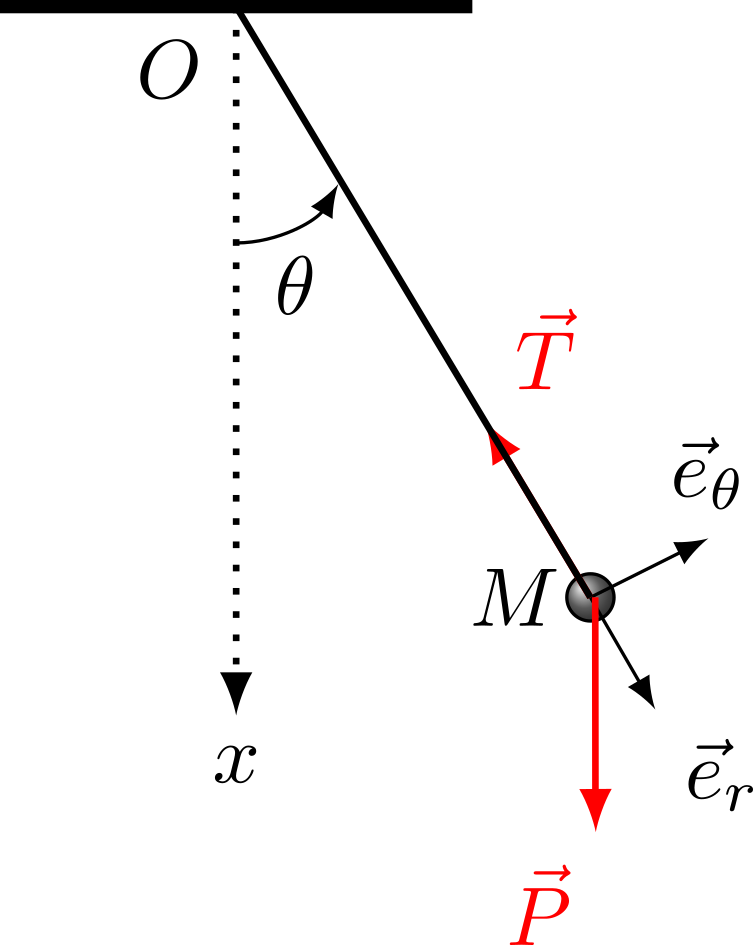
\includegraphics[width=\linewidth, draft=true]{pendule_plain}
				}{
					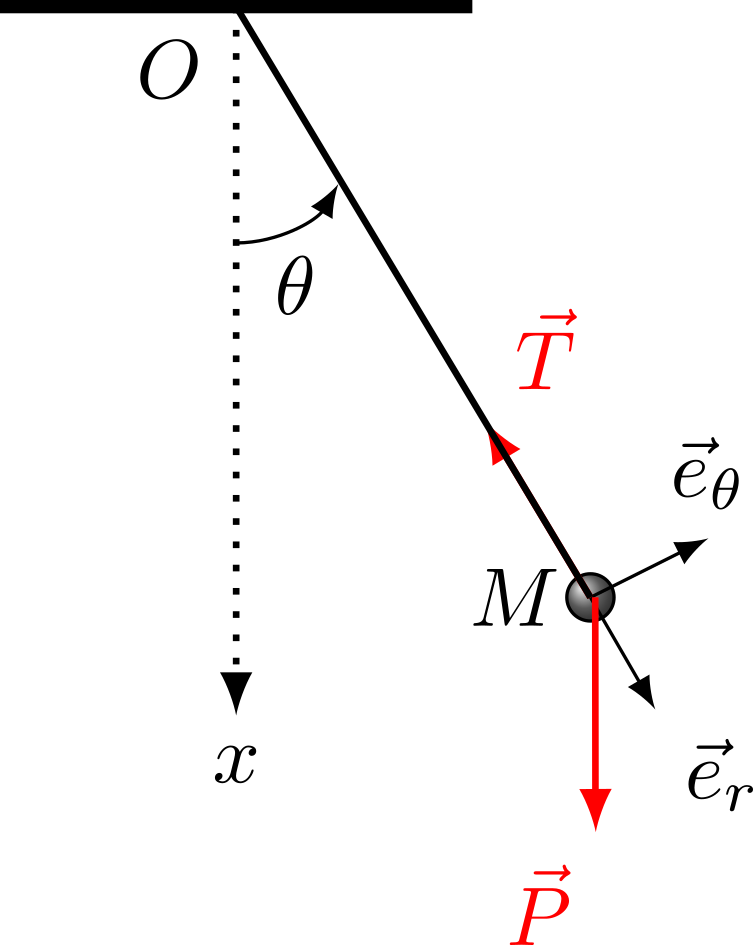
\includegraphics[width=\linewidth]{pendule_plain}
				}
				\vspace{-15pt}
				\captionsetup{justification=centering}
				\captionof{figure}{\smallbreak\ Pendule \protect\pt{1}}
			\end{center}
		\end{minipage}
		\hfill
		\begin{minipage}{0.70\linewidth}
			\psw{
				Le mouvement étant circulaire, $\vf = \ell\tp\ut$ \pt{1} et on a
				\begin{gather*}
					\Ec_c = \frac{1}{2}m\ell^2\tp^2
					\Ra
					\dv{\Ec_c}{t} = \stm{m}\ell^2\tp\tpp
				\end{gather*}
				De plus, $\vf\cdot\Tf = 0$ \pt{1} et l'angle entre $\vf$ et $\Pf$ est
				$\pi/2+\tt$~:
				\begin{gather*}
					\Pf\cdot\vf = mg\times\ell\tp\times\cos(\frac{\pi}{2}+\tt) \stm{=}
					-mg\ell\tp\sin\tt
					\\
					\cancel{m\ell^2\tp}\tpp =
					0 - \frac{
						\cancel{m}g\dcancel{\ell}\bcancel{\tp}\sin\tt
					}{
						\cancel{m}\ell^{\dcancel{2}}\tp
					}
					\Lra
					\boxed{\tpp + \frac{g}{\ell}\sin\tt \stm[-1]{=} 0}
					\vspace{-15pt}
				\end{gather*}
			}
		\end{minipage}
	\end{isd}

	\nitem{4}%
	Démontrer le théorème de l'énergie cinétique. L'appliquer pour trouver la
	vitesse d'une skieuse en bas d'une piste d'un dénivelé de hauteur $h$. On
	néglige les frottements.
	\smallbreak
	\begin{isd}[lefthand ratio=.35]
		\psw{
			\begin{DispWithArrows*}[fleqn, mathindent=10pt]
				\dv{\Ec_{c}}{t}                    & = \sum_i \Pc(\Ff_i)
				\Arrow{$\Pc = \frac{\delta W}{\dd{t}}$}
				\\\Lra
				\frac{\dd{\Ec_c}}{\cancel{\dd{t}}} & \stm{=} \sum_i \frac{\delta
					W(\Ff_i)}{\cancel{\dd{t}}}
				\CArrow{$\DS \int_{A}^{B}$}
				\\\Lra
				\Aboxed{\Delta_{\ABr}\Ec_c         & \stm[-1]{=} \sum_i W_{\ABr}(\Ff_i)}
			\end{DispWithArrows*}
		}
		\tcblower
		\psw{
			Pour la skieuse, avec A le point en haut de la piste et B en bas,
			\begin{itemize}
				\item $\Delta_{\ABr}\Ec_c = \frac{1}{2}mv^{2}$~;
				\item $W_{\ABr}(\vv{R_N}) = 0$ car $\vv{R_N} \perp \dd{\OM}$~;
				      $\quad \quad \pt{1}$
				\item $W_{\ABr}(\Pf) = mgh$.
			\end{itemize}
			Ainsi, avec le TEC entre le haut et le base de la piste, on a
			\[
				\frac{1}{2}mv^2 = mgh
				\quad\Ra\quad
				\boxed{v \stm[-1]{=} \sqrt{2gh}}
			\]
		}
	\end{isd}
	\nitem{2}%
	Comment trouver les points d'équilibre d'un système à partir de son énergie
	potentielle~? Quelle est la condition pour qu'un point d'équilibre soit
	stable~? Instable~?
	\smallbreak
	\psw{
		Les points d'équilibres se trouvent avec
		\[
			\eval{\dv{\Ec_p}{x}}_{x\ind{eq}} \stm{=} 0
		\]
		Il est stable si $\DS \eval{\dv[2]{\Ec_p}{x}}_{x\ind{eq}} > 0$, et instable
		sinon \pt{1}
	}
	\vspace*{-15pt}
	\ifstudent{
		\begin{tikzpicture}[remember picture, overlay]
			\node[anchor=north west, align=left]
			at ([shift={(1.4cm,0)}]current page.north west)
			{\\[5pt]\Large\bfseries Nom~:\\[10pt]\Large\bfseries Prénom~:};
			\node[anchor=north east, align=right]
			at ([shift={(-1.5cm,-17pt)}]current page.north east)
			{\Large\bfseries Note~:\hspace{1cm}/20};
		\end{tikzpicture}
	}
\end{enumerate}
\end{document}
